% Apresentação executiva (15 min) --- Projeto Integrador AOC 2026/02
% Compilar: latexmk -pdf slides.tex     (ou, na raiz: make paper)
\documentclass[aspectratio=169,10pt]{beamer}

\usepackage[T1]{fontenc}
\usepackage[utf8]{inputenc}
\usepackage[brazilian]{babel}
\usepackage{booktabs}
\usepackage{tikz}
\usetikzlibrary{arrows.meta,positioning}
\usepackage{pgfplots}
\usepgfplotslibrary{groupplots}
\pgfplotsset{compat=1.18}

\usetheme{default}
\usecolortheme{dove}
\setbeamertemplate{navigation symbols}{}
\setbeamertemplate{footline}[frame number]
\setbeamertemplate{itemize items}[circle]
\definecolor{tk}{RGB}{20,70,160}
\definecolor{fp}{RGB}{170,40,40}
\setbeamercolor{frametitle}{fg=tk}
\setbeamercolor{structure}{fg=tk}
\setbeamerfont{frametitle}{series=\bfseries}

\newcommand{\code}[1]{\texttt{#1}}
\newcommand{\res}{../../results}
% Gerado por: python3 -m sim.paper_numbers (não editar à mão)
\newcommand{\ERRTABLE}{T8 & \boldmath$1{,}6\times10^{0}$ & $6{,}8\times10^{-2}$ & \boldmath$2{,}1\times10^{-1}$ & $7{,}7\times10^{-2}$ & $1{,}1\times10^{-1}$ & $1{,}4\times10^{-1}$ & $5{,}7\times10^{-2}$ & \boldmath$5{,}4\times10^{-1}$ & $1{,}4\times10^{-1}$\\
FP8 & $1{,}6\times10^{0}$ & $7{,}7\times10^{-2}$ & $\infty$ & $9{,}0\times10^{-2}$ & $5{,}4\times10^{-2}$ & $6{,}4\times10^{-2}$ & $4{,}4\times10^{-2}$ & $\infty$ & $7{,}2\times10^{-2}$\\
FP8w & $1{,}7\times10^{0}$ & \boldmath$4{,}4\times10^{-2}$ & $\infty$ & \boldmath$4{,}1\times10^{-2}$ & \boldmath$3{,}8\times10^{-2}$ & \boldmath$5{,}1\times10^{-2}$ & \boldmath$3{,}6\times10^{-2}$ & $\infty$ & \boldmath$6{,}4\times10^{-2}$\\
\midrule
T16 & \boldmath$6{,}9\times10^{-3}$ & \boldmath$2{,}7\times10^{-4}$ & $8{,}4\times10^{-4}$ & \boldmath$2{,}5\times10^{-4}$ & \boldmath$2{,}6\times10^{-4}$ & $5{,}4\times10^{-4}$ & \boldmath$2{,}3\times10^{-4}$ & \boldmath$2{,}0\times10^{-3}$ & $5{,}8\times10^{-4}$\\
FP16 & $9{,}1\times10^{-3}$ & $4{,}7\times10^{-4}$ & $3{,}8\times10^{-4}$ & $6{,}7\times10^{-4}$ & $3{,}9\times10^{-4}$ & $3{,}5\times10^{-4}$ & $2{,}9\times10^{-4}$ & $\infty$ & $3{,}8\times10^{-4}$\\
FP16w & $9{,}0\times10^{-3}$ & $3{,}2\times10^{-4}$ & \boldmath$2{,}4\times10^{-4}$ & $3{,}2\times10^{-4}$ & $3{,}0\times10^{-4}$ & \boldmath$3{,}1\times10^{-4}$ & $2{,}4\times10^{-4}$ & $\infty$ & \boldmath$3{,}1\times10^{-4}$\\
\midrule
T32 & \boldmath$9{,}9\times10^{-8}$ & \boldmath$4{,}2\times10^{-9}$ & \boldmath$1{,}4\times10^{-8}$ & \boldmath$3{,}4\times10^{-9}$ & \boldmath$3{,}7\times10^{-9}$ & \boldmath$8{,}3\times10^{-9}$ & \boldmath$3{,}8\times10^{-9}$ & \boldmath$3{,}3\times10^{-8}$ & \boldmath$8{,}6\times10^{-9}$\\
FP32 & $1{,}2\times10^{-6}$ & $6{,}9\times10^{-8}$ & $5{,}2\times10^{-8}$ & $1{,}0\times10^{-7}$ & $4{,}6\times10^{-8}$ & $5{,}2\times10^{-8}$ & $3{,}7\times10^{-8}$ & $6{,}2\times10^{-8}$ & $4{,}8\times10^{-8}$\\
FP32w & $9{,}3\times10^{-7}$ & $4{,}3\times10^{-8}$ & $3{,}1\times10^{-8}$ & $3{,}8\times10^{-8}$ & $3{,}5\times10^{-8}$ & $3{,}8\times10^{-8}$ & $3{,}0\times10^{-8}$ & $4{,}0\times10^{-8}$ & $3{,}8\times10^{-8}$\\}
\newcommand{\ERRTABLESYN}{T8 & \boldmath$1{,}6\times10^{0}$ & $6{,}8\times10^{-2}$ & \boldmath$2{,}1\times10^{-1}$ & $7{,}7\times10^{-2}$\\
FP8 & $1{,}6\times10^{0}$ & $7{,}7\times10^{-2}$ & $\infty$ & $9{,}0\times10^{-2}$\\
FP8w & $1{,}7\times10^{0}$ & \boldmath$4{,}4\times10^{-2}$ & $\infty$ & \boldmath$4{,}1\times10^{-2}$\\
\midrule
T16 & \boldmath$6{,}9\times10^{-3}$ & \boldmath$2{,}7\times10^{-4}$ & $8{,}4\times10^{-4}$ & \boldmath$2{,}5\times10^{-4}$\\
FP16 & $9{,}1\times10^{-3}$ & $4{,}7\times10^{-4}$ & $3{,}8\times10^{-4}$ & $6{,}7\times10^{-4}$\\
FP16w & $9{,}0\times10^{-3}$ & $3{,}2\times10^{-4}$ & \boldmath$2{,}4\times10^{-4}$ & $3{,}2\times10^{-4}$\\
\midrule
T32 & \boldmath$9{,}9\times10^{-8}$ & \boldmath$4{,}2\times10^{-9}$ & \boldmath$1{,}4\times10^{-8}$ & \boldmath$3{,}4\times10^{-9}$\\
FP32 & $1{,}2\times10^{-6}$ & $6{,}9\times10^{-8}$ & $5{,}2\times10^{-8}$ & $1{,}0\times10^{-7}$\\
FP32w & $9{,}3\times10^{-7}$ & $4{,}3\times10^{-8}$ & $3{,}1\times10^{-8}$ & $3{,}8\times10^{-8}$\\}
\newcommand{\ERRTABLEREAL}{T8 & $1{,}1\times10^{-1}$ & $1{,}4\times10^{-1}$ & $5{,}7\times10^{-2}$ & \boldmath$5{,}4\times10^{-1}$ & $1{,}4\times10^{-1}$\\
FP8 & $5{,}4\times10^{-2}$ & $6{,}4\times10^{-2}$ & $4{,}4\times10^{-2}$ & $\infty$ & $7{,}2\times10^{-2}$\\
FP8w & \boldmath$3{,}8\times10^{-2}$ & \boldmath$5{,}1\times10^{-2}$ & \boldmath$3{,}6\times10^{-2}$ & $\infty$ & \boldmath$6{,}4\times10^{-2}$\\
\midrule
T16 & \boldmath$2{,}6\times10^{-4}$ & $5{,}4\times10^{-4}$ & \boldmath$2{,}3\times10^{-4}$ & \boldmath$2{,}0\times10^{-3}$ & $5{,}8\times10^{-4}$\\
FP16 & $3{,}9\times10^{-4}$ & $3{,}5\times10^{-4}$ & $2{,}9\times10^{-4}$ & $\infty$ & $3{,}8\times10^{-4}$\\
FP16w & $3{,}0\times10^{-4}$ & \boldmath$3{,}1\times10^{-4}$ & $2{,}4\times10^{-4}$ & $\infty$ & \boldmath$3{,}1\times10^{-4}$\\
\midrule
T32 & \boldmath$3{,}7\times10^{-9}$ & \boldmath$8{,}3\times10^{-9}$ & \boldmath$3{,}8\times10^{-9}$ & \boldmath$3{,}3\times10^{-8}$ & \boldmath$8{,}6\times10^{-9}$\\
FP32 & $4{,}6\times10^{-8}$ & $5{,}2\times10^{-8}$ & $3{,}7\times10^{-8}$ & $6{,}2\times10^{-8}$ & $4{,}8\times10^{-8}$\\
FP32w & $3{,}5\times10^{-8}$ & $3{,}8\times10^{-8}$ & $3{,}0\times10^{-8}$ & $4{,}0\times10^{-8}$ & $3{,}8\times10^{-8}$\\}
\newcommand{\RATA}{1{,}2}
\newcommand{\RATB}{11}
\newcommand{\WIDET}{$8{,}4\times10^{-4}$}
\newcommand{\WIDEF}{$2{,}4\times10^{-4}$}
\newcommand{\BUST}{$5{,}4\times10^{-4}$}
\newcommand{\BUSF}{$3{,}1\times10^{-4}$}
\newcommand{\WIDETEIGHT}{$2{,}1\times10^{-1}$}
\newcommand{\BCSTEIGHT}{$5{,}4\times10^{-1}$}
\newcommand{\BCSTSIXTEEN}{$2{,}0\times10^{-3}$}
\newcommand{\FPEIGHTBAD}{217}
\newcommand{\NFBUS}{94}
\newcommand{\NFWEST}{51}
\newcommand{\NFBCS}{153}
\newcommand{\NFWESTH}{5}
\newcommand{\NFBCSH}{149}
\newcommand{\MEMTE}{$1{,}4\times10^{-1}$}
\newcommand{\MEMTEBAD}{267}
\newcommand{\MEMFE}{$6{,}4\times10^{-2}$}
\newcommand{\MEMFEBAD}{1\,054}
\newcommand{\MEMTS}{$5{,}8\times10^{-4}$}
\newcommand{\MEMTSBAD}{3}
\newcommand{\MEMFS}{$3{,}1\times10^{-4}$}
\newcommand{\MEMFSBAD}{2}
\newcommand{\MEMTT}{$8{,}6\times10^{-9}$}
\newcommand{\MEMTTBAD}{0}
\newcommand{\MEMFT}{$3{,}8\times10^{-8}$}
\newcommand{\MEMFTBAD}{0}
\newcommand{\MEMROWS}{17\,758}
\newcommand{\MATTABLE}{poisson & 256$\times$256 & 1\,216 & 4{,}8 & $2^{0}$ -- $2^{2}$\\
gauss & 256$\times$256 & 2\,560 & 10{,}0 & $2^{-13}$ -- $2^{2}$\\
wide & 256$\times$256 & 2\,560 & 10{,}0 & $2^{-10}$ -- $2^{10}$\\
mlp & 256$\times$512 & 13\,056 & 51{,}0 & $2^{-15}$ -- $2^{0}$\\
\midrule
nos4 & 100$\times$100 & 594 & 5{,}9 & $2^{-6}$ -- $2^{-1}$\\
bus494 & 494$\times$494 & 1\,666 & 3{,}4 & $2^{-3}$ -- $2^{14}$\\
west0479 & 479$\times$479 & 1\,910 & 4{,}0 & $2^{-21}$ -- $2^{18}$\\
bcsstk05 & 153$\times$153 & 2\,423 & 15{,}8 & $2^{-31}$ -- $2^{22}$\\
memplus & 17758$\times$17758 & 126\,150 & 7{,}1 & $2^{-86}$ -- $2^{0}$\\}
\newcommand{\INSTRTABLE}{poisson & 4{,}8 & 6\,146 & 6\,146 & 6\,658 & 0{,}0\% & 7{,}7\%\\
gauss & 10{,}0 & 8\,962 & 9\,218 & 9\,986 & 2{,}8\% & 10{,}3\%\\
mlp & 51{,}0 & 23\,042 & 24\,578 & 26\,626 & 6{,}2\% & 13{,}5\%\\
\midrule
nos4 & 5{,}9 & 2\,402 & 2\,402 & 2\,602 & 0{,}0\% & 7{,}7\%\\
bus494 & 3{,}4 & 11\,902 & 11\,906 & 12\,898 & 0{,}0\% & 7{,}7\%\\
west0479 & 4{,}0 & 11\,949 & 11\,990 & 12\,989 & 0{,}3\% & 8{,}0\%\\
bcsstk05 & 15{,}8 & 6\,061 & 6\,278 & 6\,801 & 3{,}5\% & 10{,}9\%\\
memplus & 7{,}1 & 503\,161 & 510\,158 & 552\,671 & 1{,}4\% & 9{,}0\%\\}
\newcommand{\SAVEWLO}{7{,}7}
\newcommand{\SAVEWHI}{14{,}3}
\newcommand{\SAVEPHI}{7{,}1}
\newcommand{\FLAGPCT}{90}
\newcommand{\FLAGWHERE}{\emph{wide}, FP32}
\newcommand{\HWDECA}{46}
\newcommand{\HWDECB}{89}
\newcommand{\HWDECC}{164}
\newcommand{\HWENCA}{70}
\newcommand{\HWENCB}{118}
\newcommand{\HWENCC}{216}
\newcommand{\HWALUA}{327}
\newcommand{\HWALUB}{912}
\newcommand{\HWALUC}{2\,838}
\newcommand{\HWNCA}{32}
\newcommand{\HWNCB}{67}
\newcommand{\HWNCC}{155}
\newcommand{\HWWMA}{220}
\newcommand{\HWWMB}{686}
\newcommand{\HWWMC}{2\,384}
\newcommand{\HWDOTA}{6\,740}
\newcommand{\HWDOTB}{7\,525}
\newcommand{\HWDOTC}{9\,451}
\newcommand{\HWHDR}{41}

\newcommand{\cdf}[3][]{\addplot+[no markers, #1] table[x=err, y=frac] {\res/cdf_#2_#3.dat};}
\newcommand{\matplot}[2][]{%
  \nextgroupplot[title={#2}, #1]
  \cdf[blue!75!black]{#2}{T8}    \cdf[blue!75!black, dashed]{#2}{FP8w}
  \cdf[red!75!black]{#2}{T16}    \cdf[red!75!black, dashed]{#2}{FP16w}
  \cdf[green!45!black]{#2}{T32}  \cdf[green!45!black, dashed]{#2}{FP32w}}

\title{Zvtakum: aritmética takum na extensão vetorial RISC-V}
\subtitle{Projeto Integrador --- Arquitetura e Organização de Computadores 2026/02}
\author{Heloisa Silva Rosa \and Samantha Kelly de Souza Sena \and Vitor Hugo Lacerda Lana}
\institute{DELT --- UFMG}
\date{}

\begin{document}

\begin{frame}
  \titlepage
\end{frame}

%----------------------------------------------------------------------
\begin{frame}{O problema: formatos demais}
  \begin{columns}[T]
    \column{0.55\textwidth}
    \begin{itemize}
      \item Unidades vetoriais acumulam formatos IEEE de baixa precisão:\\
            binary16, bfloat16, E4M3, E5M2\ldots
      \item Cada um tem seu expoente, seus casos especiais (NaN, $\pm\infty$, $\pm0$, subnormais) e suas
            conversões.
      \item Resultado: mais instruções, mais lógica de exceção, mais estado de controle (\code{fcsr}).
    \end{itemize}
    \column{0.42\textwidth}
    \begin{block}{Takum (Hunhold, 2024)}
      \begin{itemize}
        \item Um formato para qualquer largura $n$
        \item Cabeçalho sempre nos 12 bits de cima
        \item Faixa $\approx 2^{\pm239}$ já em 8 bits
        \item Só dois especiais: $0$ e NaR
        \item Ordenado como inteiro com sinal
      \end{itemize}
    \end{block}
  \end{columns}
  \vfill
  \textbf{Pergunta do projeto:} o que isso simplifica numa extensão vetorial RISC-V, e quanto custa em precisão?
\end{frame}

%----------------------------------------------------------------------
\begin{frame}{O formato takum linear}
  \centering
  \begin{tikzpicture}[font=\small]
    \foreach \x/\w/\l/\c in {0/0.8/S/gray!25, 0.8/0.8/D/tk!25, 1.6/1.8/R (3)/tk!15, 3.4/2.6/C ($r$ bits)/orange!25, 6.0/5.0/F ($n-5-r$ bits)/green!18}
      \draw[fill=\c] (\x,0) rectangle ++(\w,0.8) node[midway] {\l};
    \draw[<->] (0,-0.25) -- node[below] {cabeçalho: no máximo 12 bits, em qualquer $n$} (6.0,-0.25);
  \end{tikzpicture}
  \[
    r = \begin{cases} R & D=1\\ 7-R & D=0\end{cases}\qquad
    c = \begin{cases} 2^r-1+C & D=1\\ -2^{r+1}+1+C & D=0\end{cases}\qquad
    x = (1+f)\cdot 2^{c}
  \]
  \begin{itemize}
    \item Precisão afunilada: perto de 1, $r=0$ e sobram $n-5$ bits de fração; nos extremos, $n-12$.
    \item Negativo = complemento de dois da palavra. \code{00\ldots0} é zero, \code{10\ldots0} é NaR.
    \item Somar 1 à palavra leva ao próximo valor representável $\Rightarrow$ arredondar é incrementar.
  \end{itemize}
\end{frame}

%----------------------------------------------------------------------
\begin{frame}{Fase 1: decodificador, codificador e ALU (Verilog)}
  \centering
  \begin{tikzpicture}[
    blk/.style={draw, rounded corners=2pt, minimum height=9mm, align=center, font=\small},
    arr/.style={-{Latex[length=2mm]}}]
    \node[blk, minimum width=26mm] (da) at (0, 0.75) {decodificador};
    \node[blk, minimum width=26mm] (db) at (0,-0.75) {decodificador};
    \node[blk, minimum width=28mm, minimum height=24mm] (core) at (4.3,0) {núcleo\\ add / sub / mul};
    \node[blk, minimum width=28mm] (enc) at (8.6,0) {codificador\\ \scriptsize arredonda e satura};
    \node (a) at (-2.3, 0.75) {$a$}; \node (b) at (-2.3,-0.75) {$b$}; \node (y) at (10.9,0) {$y$};
    \draw[arr] (a) -- (da); \draw[arr] (b) -- (db);
    \draw[arr] (da.east) -- (core.west |- da.east); \draw[arr] (db.east) -- (core.west |- db.east);
    \draw[arr] (core) -- (enc); \draw[arr] (enc) -- (y);
  \end{tikzpicture}
  \vspace{3mm}
  \begin{itemize}
    \item Um bloco fixo lê o cabeçalho de 12 bits: é o mesmo para T8, T16 e T32 (\HWHDR{} LUT6).
    \item Arredondamento para o mais próximo, empate para o par, \textbf{feito na palavra}.
    \item Um resultado não nulo nunca vira 0 nem NaR: satura.
    \item Verificação contra um oráculo exato em Python (\code{Fraction}), sem código em comum com o RTL.
          T8: todos os $65\,536$ pares $\times$ 3 operações.
  \end{itemize}
\end{frame}

%----------------------------------------------------------------------
\begin{frame}{Fase 2: a extensão Zvtakum}
  \centering\small
  \begin{tabular}{lll}
    \toprule
    Instrução & Equivalente RVV & Operação ($i<\mathit{vl}$, não mascarado)\\
    \midrule
    \code{vtadd.vv} & \code{vfadd.vv} & $vd_i = vs2_i + vs1_i$\\
    \code{vtsub.vv} & \code{vfsub.vv} & $vd_i = vs2_i - vs1_i$\\
    \code{vtmul.vv} & \code{vfmul.vv} & $vd_i = vs2_i \times vs1_i$\\
    \code{vtdot.vv} & \code{vfwmul} + redução & $vd_0$ (2\,SEW) $\mathrel{+}= \sum_i vs2_i \times vs1_i$\\
    \code{vncvt.t.t} & \code{vfncvt.f.f.w} & $vd_i$ (SEW) $=$ arredonda($vs2_i$ de 2\,SEW)\\
    \bottomrule
  \end{tabular}
  \vspace{4mm}
  \begin{itemize}
    \item Mesmo layout de campos do OP-V, no opcode \emph{custom-2}, com o \code{funct6} da instrução de ponto
          flutuante equivalente: o decodificador de um núcleo RVV é reaproveitado.
    \item SEW $= 8, 16, 32$; \code{vl}, máscara \code{v0.t} e cauda inalterada.
    \item \textbf{Nenhum estado novo}: usa só \code{vl} e \code{vtype}. Não lê nem escreve \code{fcsr}.
  \end{itemize}
\end{frame}

%----------------------------------------------------------------------
\begin{frame}{\code{vtdot.vv} e \code{vncvt.t.t}: decisões de projeto}
  \centering
  \begin{tikzpicture}[x=1.15cm, font=\footnotesize, >={Latex[length=1.6mm]},
    blk/.style={draw, rounded corners=1.5pt, minimum height=6.5mm, minimum width=14mm, align=center}]
    \foreach \i/\x in {0/0, 1/2.1, 2/4.9} {
      \node[blk] (m\i) at (\x, 0) {wmul};
      \node[blk] (a\i) at (\x,-1.2) {soma$_{2n}$};
      \draw[->] (m\i) -- (a\i);
    }
    \node at (3.5, 0) {$\cdots$}; \node at (3.5,-1.2) {$\cdots$};
    \node (in0) at (0, 0.9) {$a_0\; b_0$}; \node (in1) at (2.1, 0.9) {$a_1\; b_1$};
    \node (in2) at (4.9, 0.9) {$a_{k-1}\; b_{k-1}$};
    \foreach \i in {0,1,2} \draw[->] (in\i) -- (m\i);
    \node (acc) at (-1.5,-1.2) {$vd_0$};
    \draw[->] (acc) -- (a0); \draw[->] (a0) -- (a1);
    \draw[->] (a1) -- (2.95,-1.2); \draw[->] (4.05,-1.2) -- (a2);
    \node[blk] (nc) at (6.9,-1.2) {ncvt};
    \draw[->] (a2) -- node[above] {$2n$} (nc);
    \node (y) at (8.4,-1.2) {$n$ bits};
    \draw[->] (nc) -- (y);
  \end{tikzpicture}
  \vspace{2mm}
  \begin{itemize}
    \item \textbf{Produto em $2n$ bits é exato:} o produto dos significandos ($2n-8$ bits) sempre cabe na fração
          do takum de $2n$ bits. Conferido para todos os pares de T8.
    \item \textbf{Acúmulo em precisão ampliada:} só as somas arredondam, e em $2n$ bits.
          O acumulador fica em \code{vd}: o laço não precisa de redução nem de \code{vsetvli} extra.
    \item \textbf{Estreitar é arredondar a palavra:} o cabeçalho está no topo em qualquer largura.
          \code{vncvt.t.t} custa \HWNCA{} / \HWNCB{} / \HWNCC{} LUT6, menos que um decodificador.
    \item Alternativa descartada: acumulador exato de ponto fixo (\emph{quire}); com faixa $2^{\pm255}$
          teria mais de mil bits.
  \end{itemize}
\end{frame}

%----------------------------------------------------------------------
\begin{frame}{\code{vncvt.t.t}: o circuito e as ondas}
  \centering
  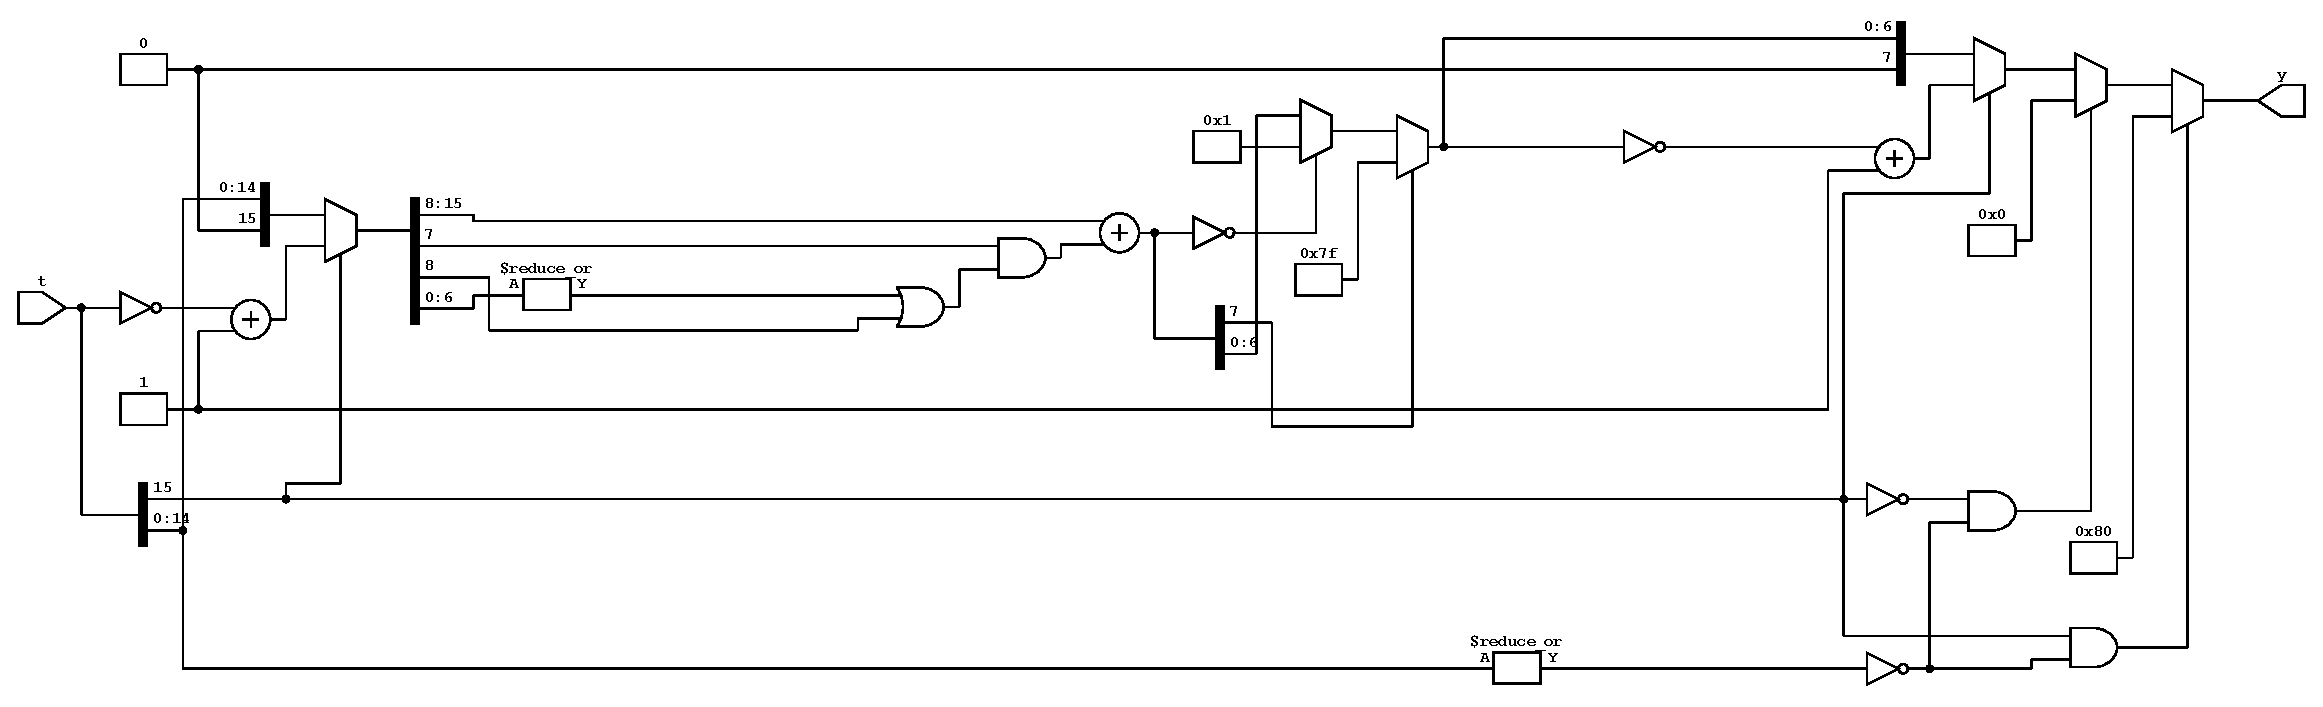
\includegraphics[width=0.86\linewidth]{../img/takum_ncvt.pdf}\\[1mm]
  {\scriptsize Esquemático gerado do Verilog (Yosys + netlistsvg): nega, corta, arredonda com um somador, satura. Sem decodificador.}\\[3mm]
  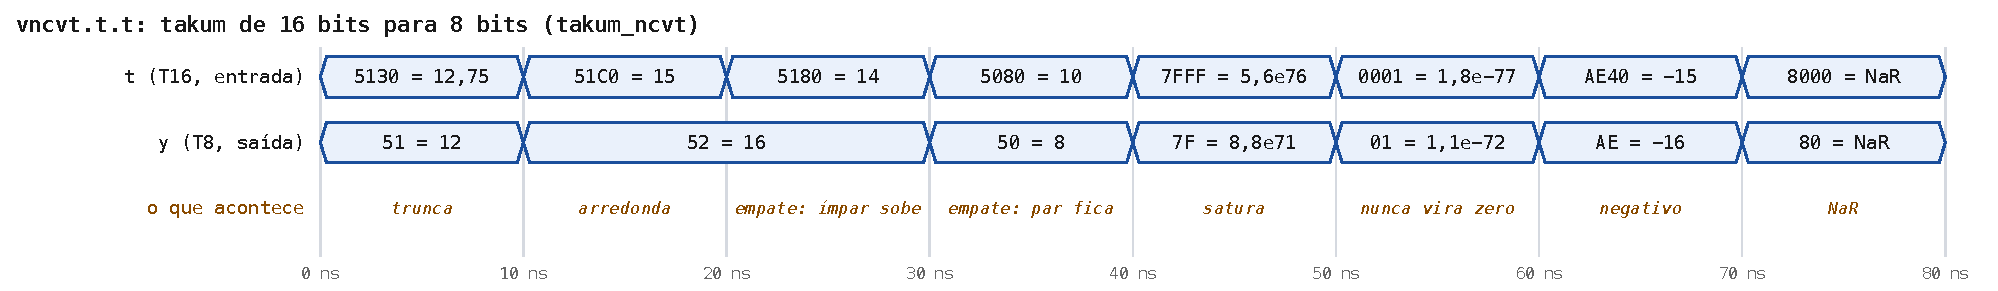
\includegraphics[width=\linewidth]{../img/ondas-fase2-ncvt.pdf}
\end{frame}

%----------------------------------------------------------------------
\begin{frame}{\code{vtdot.vv} funcionando na unidade vetorial}
  \centering
  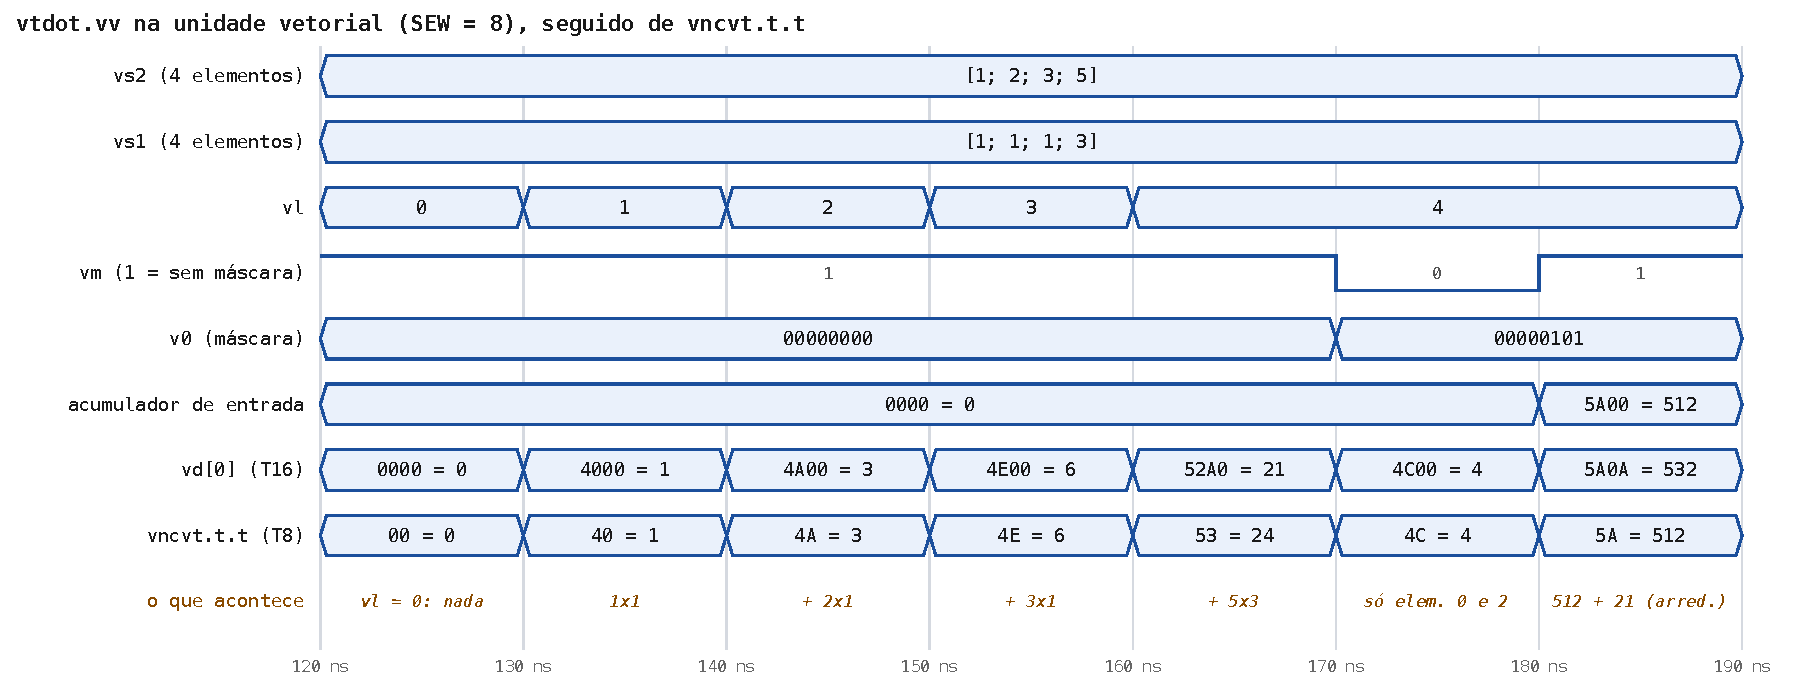
\includegraphics[width=0.93\linewidth]{../img/ondas-fase2-vtdot.pdf}\\[1.5mm]
  {\footnotesize $[1;2;3;5]\cdot[1;1;1;3]$: o acumulador \code{vd[0]} cresce com \code{vl} (1, 3, 6, 21); com a máscara \code{101} entram só $1+3$.\\
  Simulação do Verilog (\code{make waves2}); o esquemático do circuito está em \code{docs/img/takum\_dot.svg} (\code{make schematic}).}
\end{frame}

%----------------------------------------------------------------------
\begin{frame}{Verificação}
  \begin{columns}[T]
    \column{0.56\textwidth}
    \small
    \begin{tabular}{@{}lr@{}}
      \toprule
      Teste (RTL $\times$ oráculo exato) & Vetores\\
      \midrule
      Decodificador, codificador, ida e volta & 855\,408\\
      ALU T8: todos os pares $\times$ 3 operações & 196\,608\\
      ALU T16 e T32 (cada) & 109\,923\\
      \code{vncvt.t.t} (T16$\to$T8 completo) & 105\,794\\
      Produto alargado (T8 completo) & 138\,818\\
      Unidade vetorial, por SEW & 5\,000\\
      \bottomrule
    \end{tabular}
    \column{0.42\textwidth}
    \begin{itemize}
      \item \code{make test}: tudo passa.
      \item Conferido contra a \textbf{libtakum}, do autor do formato: 826\,987 vetores iguais; 16 produtos
            T32 diferem no último bit por limite do \code{double} dela.
      \item 13 defeitos injetados de propósito (sem \emph{sticky}, sem empate para o par, máscara ignorada,
            ordem do acúmulo\ldots): \textbf{todos detectados}.
      \item Simulador: IEEE conferido contra o ponto flutuante nativo; os $15\,000$ vetores do RTL rodam
            como instruções codificadas e dão o mesmo resultado.
    \end{itemize}
  \end{columns}
\end{frame}

%----------------------------------------------------------------------
\begin{frame}[fragile]{Modelo de simulação RVV (Python)}
  \begin{columns}[T]
    \column{0.47\textwidth}
    \begin{itemize}
      \item Monta, codifica em 32 bits, decodifica e executa: RV64I mínimo, subconjunto de RVV 1.0 e Zvtakum.
      \item Conta instruções executadas e os \code{fflags} levantados.
      \item IEEE genérico corretamente arredondado: FP8 (E4M3), binary16, bfloat16, binary32/64/128.
      \item Takum: o mesmo oráculo que verifica o RTL.
      \item Demonstração: \code{make simdemo}
    \end{itemize}
    \column{0.5\textwidth}
\begin{verbatim}
inner:
  vsetvli    t3, t2, e16, m1, ta, ma
  vle32.v    v8, (a2)      # colunas
  vle16.v    v1, (a3)      # valores
  vluxei32.v v2, (a4), v8  # x[col]
  vtdot.vv   v4, v1, v2    # T32 += v1.v2
  ...
done:
  vncvt.t.t  v5, v4        # T32 -> T16
  vse16.v    v5, (a5)
\end{verbatim}
    \footnotesize Laço interno de $y = Ax$ (CSR) com Zvtakum.
  \end{columns}
\end{frame}

%----------------------------------------------------------------------
\begin{frame}{Fase 3: erro relativo de $y = Ax$ contra Float128}
  \centering
  \begin{tikzpicture}
  \begin{groupplot}[
    group style={group size=5 by 2, horizontal sep=4mm, vertical sep=9mm, ylabels at=edge left,
                 yticklabels at=edge left, xlabels at=edge bottom},
    width=0.232\textwidth, height=31mm,
    xmode=log, xmin=1e-10, xmax=1e2, ymin=0, ymax=1,
    xtick={1e-10,1e-8,1e-6,1e-4,1e-2,1e0,1e2},
    xticklabels={,,$10^{-6}$,,,$10^{0}$,},
    ytick={0,0.5,1}, yticklabels={0,{0,5},1},
    xlabel={erro relativo}, ylabel={fração das linhas},
    grid=major, grid style={black!12},
    tick label style={font=\tiny}, label style={font=\scriptsize}, title style={font=\scriptsize, yshift=-2mm},
    cycle list={}, every axis plot/.append style={line width=0.9pt},
    legend style={font=\scriptsize, legend columns=6, draw=none, /tikz/every even column/.append style={column sep=3mm}}]
  \matplot{poisson}
  \matplot{gauss}
  \matplot{wide}
  \matplot{mlp}
  \matplot{nos4}
  \matplot{bus494}
  \matplot{west0479}
  \matplot{bcsstk05}
  \matplot[legend to name=cdfleg]{memplus}
  \legend{T8, FP8w, T16, FP16w, T32, FP32w}
  \end{groupplot}
  \end{tikzpicture}\\[0.5mm]
  \pgfplotslegendfromname{cdfleg}

  \vspace{0.5mm}\scriptsize
  Contínuo: takum (\code{vtdot.vv}). Tracejado: IEEE com o mesmo acúmulo ampliado. Mais à esquerda é melhor.
  Curva que não chega a 1: $\infty$ ou NaN.\\
  Quatro matrizes geradas e cinco reais do Matrix Market (NIST): viga, rede elétrica, coluna de destilação,
  rigidez estrutural e \code{memplus}, um circuito de memória com 17\,758 linhas.
\end{frame}

%----------------------------------------------------------------------
\begin{frame}{O que os erros mostram}
  \centering\scriptsize
  \setlength{\tabcolsep}{2.5pt}
  \resizebox{\linewidth}{!}{%
  \begin{tabular}{@{}lccccccccc@{}}
    \toprule
    Erro mediano & poisson & gauss & wide & mlp & nos4 & bus494 & west0479 & bcsstk05 & memplus\\
    \midrule
    \ERRTABLE
    \bottomrule
  \end{tabular}}
  \vspace{1.5mm}
  \small
  \begin{itemize}
    \item \textbf{32 bits:} T32 ganha nas nove matrizes, de \RATA{} a \RATB{} vezes.
    \item \textbf{16 bits:} T16 ganha perto da escala unitária, \textbf{perde} em faixa moderada
          (\code{wide}, \code{bus494}, \code{memplus}: 8 bits de fração contra 10) e continua respondendo onde o binary16
          estoura (\NFBCSH{} de 153 linhas de \code{bcsstk05}).
    \item \textbf{8 bits:} dentro da faixa o FP8 é \textbf{mais preciso} (1,5 a 3 vezes). Mas ele devolve
          $\infty$ ou NaN em 4 das 9 matrizes (\FPEIGHTBAD/256, \NFBUS/494, \NFWEST/479, \NFBCS/153); o T8,
          em nenhuma linha.
  \end{itemize}
\end{frame}

%----------------------------------------------------------------------
\begin{frame}{Contagem de instruções e CSRs}
  \begin{columns}[T]
    \column{0.52\textwidth}
    \centering\scriptsize
    \setlength{\tabcolsep}{3pt}
    \begin{tabular}{@{}lrrrrrr@{}}
      \toprule
       & nnz/ & & & & \multicolumn{2}{c}{Economia vs.}\\
      Matriz & linha & Zvtakum & FP & FPw & FP & FPw\\
      \midrule
      \INSTRTABLE
      \bottomrule
    \end{tabular}\\[1mm]
    \footnotesize Instruções executadas, SEW $=16$, VLEN $=128$.
    \column{0.46\textwidth}
    \small
    \begin{itemize}
      \item Laço interno: 11 instruções com \code{vtdot.vv}, 12 com \code{vfmul}+\code{vfredosum}, 13 com alargamento.
            O ganho cresce com os não nulos por linha.
      \item \textbf{CSR:} IEEE usa \code{frm} (3 bits) e \code{fflags} (5 bits); até \FLAGPCT\% das operações
            levantaram algum flag. Takum: um modo de arredondamento, NaR em banda, \textbf{zero bits de CSR}.
      \item \textbf{Viram operações inteiras:} 6 comparações (\code{vmf*}), \code{vfmin}/\code{vfmax},
            \code{vfsgnj*}, \code{vfclass}.
      \item \textbf{Conversões:} estreitar = arredondar a palavra; alargar = acrescentar zeros.
    \end{itemize}
  \end{columns}
\end{frame}

%----------------------------------------------------------------------
\begin{frame}{Custo de hardware (Yosys, LUT6, síntese genérica)}
  \centering
  \begin{tabular}{lrrr}
    \toprule
    Bloco & T8 & T16 & T32\\
    \midrule
    Decodificador & \HWDECA & \HWDECB & \HWDECC\\
    Codificador & \HWENCA & \HWENCB & \HWENCC\\
    ALU (add, sub, mul) & \HWALUA & \HWALUB & \HWALUC\\
    \code{vncvt.t.t} (para esta largura) & \HWNCA & \HWNCB & \HWNCC\\
    Multiplicador com alargamento & \HWWMA & \HWWMB & \HWWMC\\
    \code{vtdot.vv}, vetor de 64 bits (8/4/2 pistas) & \HWDOTA & \HWDOTB & \HWDOTC\\
    \bottomrule
  \end{tabular}
  \vspace{3mm}
  \begin{itemize}
    \item Servem para comparar os blocos entre si, não como área absoluta.
    \item O \code{vtdot.vv} combinacional é caro: uma soma de $2n$ bits por pista. Numa implementação real,
          um somador iterado por ciclo.
    \item Em 32 bits o multiplicador $28\times28$ domina.
  \end{itemize}
\end{frame}

%----------------------------------------------------------------------
\begin{frame}{Conclusões}
  \begin{itemize}
    \item O cabeçalho fixo de 12 bits dá \textbf{um decodificador para todas as larguras}.
    \item Padrões monótonos transformam arredondamento, estreitamento, comparação e negação em
          \textbf{operações inteiras}.
    \item Sem flags e sem modos de arredondamento: \textbf{nenhum CSR de ponto flutuante}.
    \item Numericamente (9 matrizes, 5 reais, uma com 17\,758 linhas): melhor em 32 bits; em 16 bits, melhor perto da escala
          unitária; em 8 bits o ganho é a faixa, não a precisão.
    \item O produto escalar fundido encurta o SpMV em 8--14\% frente ao núcleo IEEE de mesma precisão.
  \end{itemize}
  \vspace{2mm}
  \textbf{Limitações e próximos passos}
  \begin{itemize}
    \item Caminho de dados combinacional, sem temporização; falta comparar área com uma ALU IEEE.
    \item Só uma matriz grande; o simulador conta instruções, não ciclos.
  \end{itemize}
  \vfill
  \footnotesize \code{rtl/} \;$\cdot$\; \code{tb/} \;$\cdot$\; \code{sim/} \;$\cdot$\; \code{results/} \qquad \code{make test} \;$\cdot$\; \code{make bench} \;$\cdot$\; \code{make simdemo}
\end{frame}

\end{document}
